\section{Скалярное, векторное и смешанное произведения}

\subsection{Скалярное произведение}

\begin{definition}
    \textit{Скалярное произведение} c = $(\overline{a}, \overline{b})$ определяется по следующим правилам:

    \begin{enumerate}
        \item Если $\overline{a}$ = 0 или $\overline{b}$ = 0, то с = 0
        \item Если $\overline{a}$ $\neq$ 0 и $\overline{b}$ $\neq$ 0, то с = $|\overline{a}|\cdot|\overline|b|\cdot cos(\overline{a}, \overline{b})$
    \end{enumerate}
\end{definition}

\textit{Свойства скалярного произведения:}

\begin{enumerate}
    \item ($\overline{a}, \overline{b}$) = 0 $\longleftrightarrow$
    $\begin{gathered}
        \overline{a} = \overline{0}\\
        \overline{b} = \overline{0}\\
        \overline{a} \perp \overline{b}\\
    \end{gathered}$
    \item $\forall\overline{a}, \overline{b}\hookrightarrow(\overline{a}, \overline{b}) = (\overline{b}, \overline{a})$
    \item $\forall\overline{a}$    $(\overline{a}, \overline{a}) = |\overline{a}|^2\geq0$ $-$ скалярный квадрат
    \item $\forall\overline{a}$    $(\overline{a}, \overline{a}) = 0 \longleftrightarrow \overline{a} = \overline{0}$
\end{enumerate}

\begin{lemma}
    Пусть $\overline{a}$ $-$ фиксированный вектор, тогда $\forall\overline{x}$
    \begin{center}
        ($\overline{a}, \overline{x}$) = 0 $\longrightarrow \overline{a} = \overline{0}$
    \end{center}
\end{lemma}

Для векторов ортонормированного базиса:
\begin{center}
    ($\overline{e_i}, \overline{e_j}$) = 
    $\begin{cases}
        0, i \neq  j\\
        1, i = j\\
    \end{cases}$
\end{center}

Пусть базис $\overline{e_1}, \overline{e_2}, \overline{e_3}$ $-$ ортогональный, тогда координаты вектора $\overline{a}$ находятся по формулам:

\begin{center}
    $a_1$ = $\dfrac{(\overline{a}, \overline{e_1})}{|\overline{e_1}|^2 }$, $a_2$ = $\dfrac{(\overline{a}, \overline{e_2})}{|\overline{e_2}|^2 }$, $a_3$ = $\dfrac{(\overline{a}, \overline{e_3})}{|\overline{e_3}|^2 }$
\end{center}

В ортонормированном базисе:

\begin{center}
    $\overline{a}$ = $(\overline{a}, \overline{e_1})\overline{e_1} + (\overline{a}, \overline{e_2})\overline{e_2} + (\overline{a}, \overline{e_3})\overline{e_3}$
\end{center}

\begin{theorem}
    \textit{Свойство линейности скалярного произведения:}
    \begin{center}
        $\forall\alpha,\beta\in\R, \forall\overline{a}, \overline{b}, \overline{c}$\\
        $(\alpha\overline{a} + \beta\overline{b}, \overline{c})$ = $\alpha(\overline{a}, \overline{c}) + \beta(\overline{b}, \overline{c})\tab(1)$\\
        $(\overline{c}, \alpha\overline{a} + \beta\overline{b})$ = $\alpha(\overline{c}, \overline{a}) + \beta(\overline{c}, \overline{b})\tab(2)$
    \end{center}
\end{theorem}
\begin{proof}
    (2) следует из (1), поэтому докажем только (1)\\

    Рассмотрим случаи.
    
    \begin{enumerate}
        \item $\overline{c} = \overline{0} \longrightarrow$ утверждение верно
        \item $\overline{c} \neq \overline{0} \longrightarrow$ Рассмотрим ортогональный базис, в котороом $\overline{c}$ = $\overline{e_1}$. Докажем равенство, эквивалентное (1):
        \[
        \dfrac{(\alpha\overline{a} + \beta\overline{b}, \overline{c})}{|\overline{c}|^2} = \dfrac{\alpha(\overline{a}, \overline{c})}{|\overline{c}|^2} + \dfrac{\beta(\overline{b}, \overline{c})}{|\overline{c}|^2}
        \]
        Слева первая координата вектора $\alpha\overline{a} + \beta\overline{b}$ в базисе.\\
        Справа также первая координата ветора $\alpha\overline{a} + \beta\overline{b}$ в базисе $\longrightarrow$ ч.т.д.
    \end{enumerate}
\end{proof}

\begin{corollary}
    Если в каком-то базисе у векторов равные координаты, то данные векторы равны в любом базисе.
\end{corollary}

Пусть имеется двумерный базис $\overline{e_1}$, $\overline{e_2}$, $\overline{a}(a_1, a_2)$, $\overline{b}(b_1, b_2)$, тогда
\[
(\overline{a}, \overline{b}) = (a_1\overline{e_1} + a_2\overline{e_2}, b_1\overline{e_1} + b_2\overline{e_2}) = a_1 b_1(\overline{e_1}, \overline{e_1}) + a_1 b_2(\overline{e_1}, \overline{e_2}) + a_2 b_1(\overline{e_2}, \overline{e_1}) + a_2 b_2(\overline{e_2}, \overline{e_2})
\]
Аналогично для трехмерного пространства.\\

\begin{theorem}
    Рассмотрим базис $\overline{e_1}, \overline{e_2}, \overline{e_3}$. Тройка $\overline{e_1}*, \overline{e_2}*, \overline{e_3}*$ определяется однозначно и образует базис, если она является $\textit{биортогональным (взаимным)}$ базисом, т.е. выполняется следующее условие
    \[
    (\overline{e_i}, \overline{e_j}*) = 
    \begin{cases}
        0, i \neq  j\\
        1, i = j\\
    \end{cases}
    \]
\end{theorem}

\begin{proof}
    \tab\\
    \begin{enumerate}
        \item Определяется однозначно.\\
            
        $\overline{e_1}* \perp \overline{e_2}, \overline{e_3}$\\
        $\overline{e_1}$ направлен в то же полупространство, что и $\overline{e_1}*$ $\longrightarrow$ $(\overline{e_1}*, \overline{e_1})$ определено однозначно $\longrightarrow$ |$\overline{e_1}*$| определено однозначно.\\
        Аналогично для $\overline{e_2}*, \overline{e_3}*$ $\longrightarrow$ ч.т.д.

        \item Образует базис.\\

        Пусть $\overline{x}$ раскладывается по $\overline{e_1}*, \overline{e_2}*, \overline{e_3}*$ $\longrightarrow$ $\overline{x} = \alpha_1\overline{e_1}* + \alpha_2\overline{e_2}* + \alpha_3\overline{e_3}*$\\
        Скаляроне умножение на $\overline{e_1}$: ($\overline{x}, \overline{e_1}$) = $\alpha_1(\overline{e_1}, \overline{e_1}*) + \alpha_2(\overline{e_2}, \overline{e_2}*) + \alpha_3(\overline{e_3}, \overline{e_3}*)$, что по определению равно $\alpha_1$ $\longrightarrow$ $\alpha_1$ определяется однозначно.

        Аналогично для $\alpha_2$ и $\alpha_3$, значит, по теореме о линейной независимости, ч.т.д.
    \end{enumerate}
\end{proof}

\begin{corollary}
    \tab\\
    \begin{enumerate}
        \item Для $\overline{e_1}*, \overline{e_2}*, \overline{e_3}*$ базис $\overline{e_1}, \overline{e_2}, \overline{e_3}$ $-$ биортогональный.
        \item Ортонормированный базис взаимен самому себе.
        \item Пусть известны координаты $\overline{a}(a_1, a_2, a_3)$ в базисе $\overline{e_1}, \overline{e_2}, \overline{e_3}$ и $\overline{b}(b_1, b_2, b_3)$ в базисе $\overline{e_1}*, \overline{e_2}*, \overline{e_3}*$ $\longrightarrow$
        \[
        (\overline{a}, \overline{b}) = \alpha_1 \beta_1* + \alpha_2 \beta_2* + \alpha_3 \beta_3*
        \]
    \end{enumerate}
\end{corollary}

\textbf{Нахождение проекции вектора}\\
\begin{wrapfigure}{l}{0.4\textwidth}
	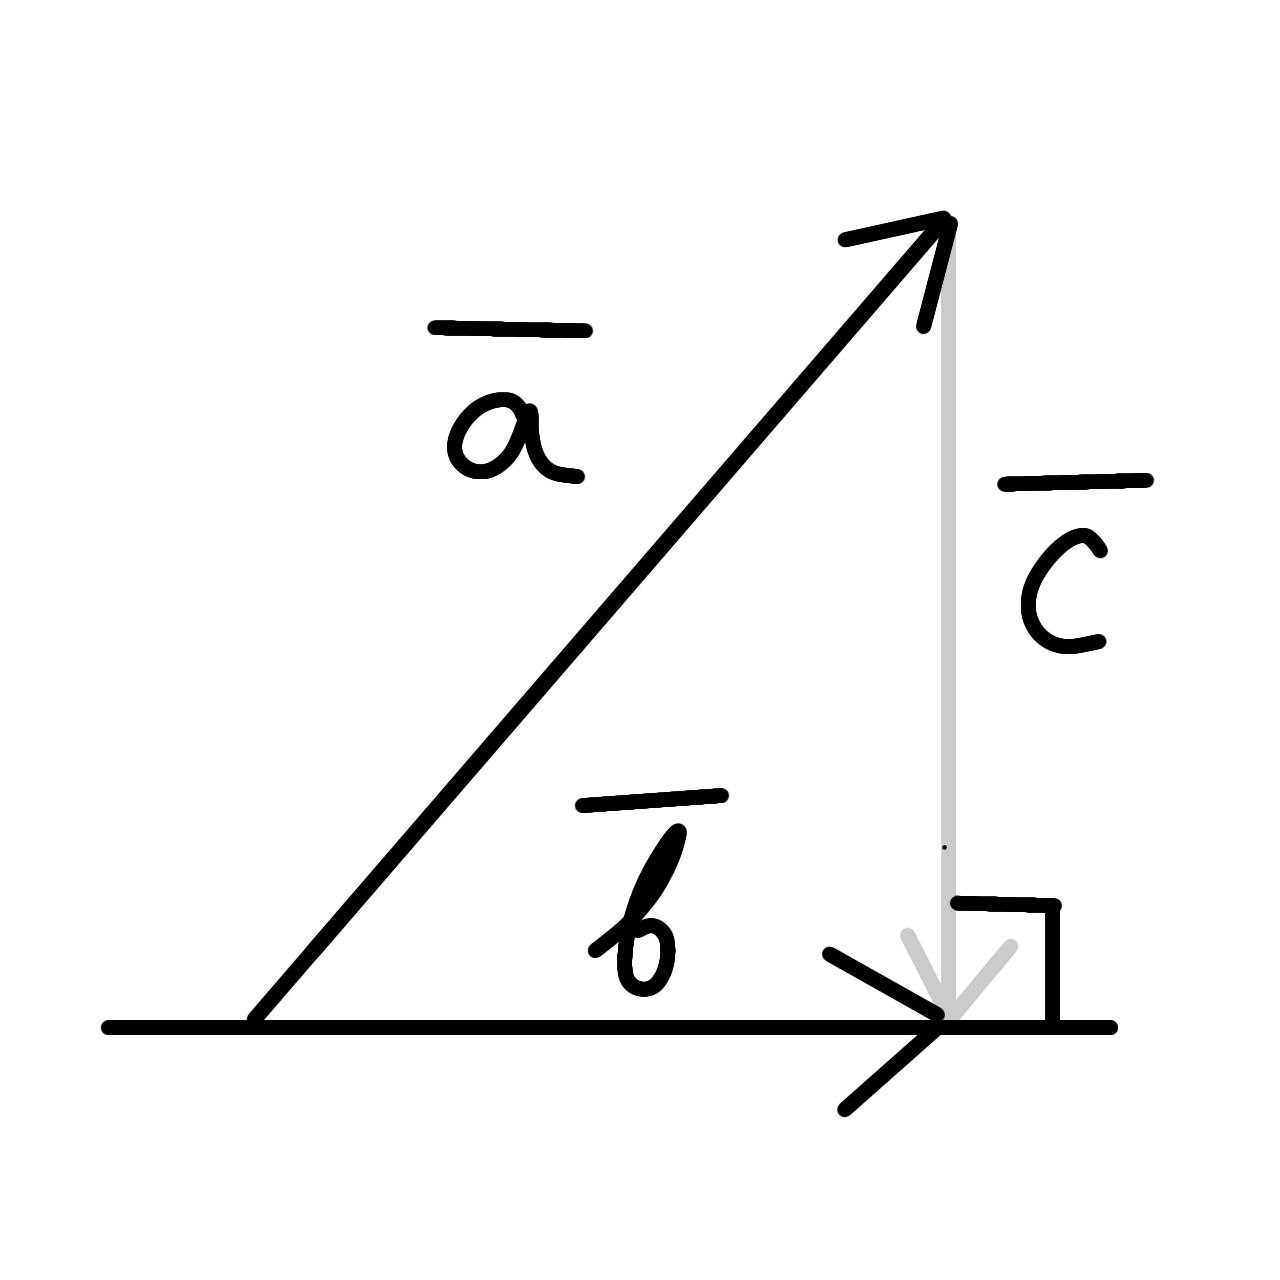
\includegraphics[width=0.84\linewidth]{images/проекция.jpeg}
\end{wrapfigure}

Пусть $\overline{a}$ $-$ вектор, который проецируем, $\overline{b}$ $-$ вектор, на который проецируем, $\overline{c}$ $-$ ортогональная составляющая.

\[
\text{Пр}_{\overline{b}}^{\overline{a}} = |\overline{a}| \cdot cos\thinspace\phi \cdot \dfrac{\overline{b}}{|\overline{b}|} = \dfrac{(\overline{a}, \overline{b})}{|\overline{b}|^2}\overline{b},
\]

где $\dfrac{(\overline{a}, \overline{b})}{|\overline{b}|^2}$ $-$ численное значение проекции

\tab\\ \tab\\ \tab\\ \tab\\

\subsection{Векторное произведение}

\begin{definition}
    Упорядоченную тройку векторов $\overline{a}, \overline{b}, \overline{c}$ назовем $\textit{правой}$, если при рассмотрении из полупространства, в которое направлен вектор $\overline{c}$ крачайший поворот от $\overline{a}$  к $\overline{b}$ направлен против часовой стрелки.\\

    Иначе $\overline{a}, \overline{b}, \overline{c}$ $-$ $\textit{левая}$ тройка.
\end{definition}

Если $\overline{a}, \overline{b}, \overline{c}$ $-$ правая, то $\overline{c}, \overline{a}, \overline{b}$ $-$ правая, а $\overline{b}, \overline{a}, \overline{c}$ $-$ левая.

\begin{definition}
    $\textit{Векторное произведение}$ $\overline{a}$ и $\overline{b}$  $\overline{c} = [\overline{a}, \overline{b}]$ определяется следующим образом:
    \begin{enumerate}
        \item если $\overline{a}$ и $\overline{b}$ $-$ коллинеарные (включая $\overline{0}$), то $\overline{c} = 0$
        \item если $\overline{a}$ и $\overline{b}$ $-$ неколлинеарные, то 
        \begin{itemize}
            \item $|\overline{c}| = |\overline{a}|\cdot|\overline{b}|\cdot sin(\overline{a}, \overline{b})$
            \item $\overline{a}\perp\overline{c}$, $\overline{b}\perp\overline{c}$
            \item $\overline{a}, \overline{b}, \overline{c}$ $-$ правая тройка
        \end{itemize}
    \end{enumerate}
\end{definition}

\textit{Свойства векторного произведения:}

\begin{enumerate}
    \item $[\overline{a}, \overline{b}]$ = $\overline{0}$ $\longleftrightarrow$ $\overline{a}$ и $\overline{b}$ $-$ коллинеарные
    \item $\forall\overline{a}, \overline{b}$ $[\overline{a}, \overline{b}] = - [\overline{b}, \overline{a}]$
    \item $|[\overline{a}, \overline{b}]|$ $-$ площадь параллелограмма, построенного на векторах $\overline{a}, \overline{b}$
    \item Свойство линейности векторного произведени:
    \[
    \forall\alpha, \beta \in \R\tab\forall\overline{a}, \overline{b}, \overline{c}\hookrightarrow[\alpha\overline{a} + \beta\overline{b}, \overline{c}] = \alpha[\overline{a}, \overline{c}] + \beta[\overline{b}, \overline{c}]
    \]
\end{enumerate}

Пусть известны базис $\overline{e_1}, \overline{e_2}, \overline{e_3}$, $\overline{a}(a_1, a_2, a_3)$, $\overline{b}(b_1, b_2, b_3)$ $\longrightarrow$ 

\begin{center}
    $[\overline{a}, \overline{b}]$ = $[a_1\overline{e_1} + a_2\overline{e_2} + a_3\overline{e_3}, b_1\overline{e_1} + b_2\overline{e_2} + b_3\overline{e_3}]$ = $\sum a_i b_j [\overline{e_i}, \overline{e_j}]$ = $[\overline{e_1}, \overline{e_2}](a_1 b_2 - a_2 b_1) + [\overline{e_2}, \overline{e_3}](a_2 b_3 - a_3 b_2) + [\overline{e_3}, \overline{e_1}](a_3 b_1 - a_1 b_3)$ = 
    $\begin{vmatrix}
        [\overline{e_2}, \overline{e_3}] & [\overline{e_3}, \overline{e_1}] & [\overline{e_1}, \overline{e_2}]\\
        a_1 & a_2 & a_3\\
        b_1 & b_2 & b_3\\
    \end{vmatrix}$
\end{center}

В правом ОНБ:
\[
    [\overline{a}, \overline{b}] = 
    \begin{vmatrix}
        \overline{e_1} & \overline{e_2} & \overline{e_3}\\
        a_1 & a_2 & a_3\\
        b_1 & b_2 & b_3\\
    \end{vmatrix}
\]
\subsection{Смешанное произведение}

\begin{definition}
    \textit{Смешанное произведение} векторов $\overline{a}, \overline{b}, \overline{c}$ определяется как 
    \[
    (\overline{a}, \overline{b}, \overline{c}) = ([\overline{a}, \overline{b}], \overline{c})
    \]
\end{definition}

\begin{theorem}
    Смешенное произведение равно объему ориентированного параллелепипеда, построенного на векторах $\overline{a}, \overline{b}, \overline{c}$
\end{theorem}

\begin{proof}
    \tab\\
    \begin{enumerate}
        \item $\overline{a}, \overline{b}$ $-$ коллинеарны $\longrightarrow$ 
        $\begin{cases}
            (\overline{a}, \overline{b}, \overline{c}) = 0\\
            V = 0\\
        \end{cases}$
        \item $\overline{a}, \overline{b}$ $-$ неколлинеарны
        \begin{itemize}
            \item $\overline{a}, \overline{b}, \overline{c}$ $-$ компланарны $\longrightarrow$
            $\begin{cases}
                (\overline{a}, \overline{b}, \overline{c}) = 0\\
                V = 0\\
            \end{cases}$
            \item $\overline{a}, \overline{b}, \overline{c}$ $-$ некомпланарны $\longrightarrow$
            \[
            V = S_{\text{осн}}\cdot h = |[\overline{a}, \overline{b}]|\cdot|\overline{c}|\cdot|cos\thinspace\phi| = |(\overline{a}, \overline{b}, \overline{c})|
            \]
        \end{itemize}
    \end{enumerate}
\end{proof}

\textit{Свойства смешанного произведения:}

\begin{enumerate}
    \item $(\overline{a}, \overline{b}, \overline{c})$ = $(\overline{b}, \overline{c}, \overline{a})$ = $(\overline{c}, \overline{a}, \overline{b})$ = -$(\overline{a}, \overline{c}, \overline{b})$ = -$(\overline{b}, \overline{a}, \overline{c})$ = -$(\overline{c}, \overline{b}, \overline{a})$
    \begin{corollary}
        $([\overline{a}, \overline{b}], \overline{c})$ = $(\overline{a}, [\overline{b}, \overline{c}])$
    \end{corollary}
    \item Линейность смешанного произведения:
    \[
    \forall\alpha_1, \alpha_2\tab\forall\overline{a_1}, \overline{a_2}, \overline{b}, \overline{c}\hookrightarrow (\alpha_1\overline{a_1} + \alpha_2\overline{a_2}, \overline{b}, \overline{c}) = \alpha_1(\overline{a_1}, \overline{b}, \overline{c}) + \alpha_2(\overline{a_2}, \overline{b}, \overline{c})
    \]
\end{enumerate}

\begin{theorem}
    \[
    [\overline{a}, \overline{b}], [\overline{b}, \overline{c}], [\overline{c}, \overline{a}] - \text{линейно независимые} \longleftrightarrow \overline{a}, \overline{b}, \overline{c} - \text{линейно независимые}
    \]
\end{theorem}
\begin{proof}
    \tab\\
    \begin{enumerate}
        \item $\overline{a}, \overline{b}, \overline{c}$ - компланарные $\longrightarrow$ векторные произведения или равны $\overline{0}$, или перпендикулярны векторам $\longrightarrow$ линейно зависимые
        \item $\overline{a}, \overline{b}, \overline{c}$ - некомпланарные $\longrightarrow$ $\exists \alpha,\beta,\gamma$ :
        \[
        \alpha[\overline{a}, \overline{b}] + \beta[\overline{b}, \overline{c}] + \gamma[\overline{c}, \overline{a}] = \overline{0}
        \]
        Скалярно домножим на $\overline{a}$ и получим
        \[
        0 + \beta(\overline{a}, \overline{b}, \overline{c}) + 0 = 0
        \]
        $\overline{a}, \overline{b}, \overline{c}$ $-$ некомпланарны $\longrightarrow$ $(\overline{a}, \overline{b}, \overline{c})\neq 0$ $\longrightarrow$ $\beta$ = 0, аналогично для $\alpha$ и $\gamma$ $\longrightarrow$ $\alpha=\beta=\gamma=0$ $-$ тривиальная комбинация $\longrightarrow$ $[\overline{a}, \overline{b}], [\overline{b}, \overline{c}], [\overline{c}, \overline{a}]$ $-$ линейно независимые
        
    \end{enumerate}
\end{proof}

\begin{corollary}
    Попарные векторные произведения линейно независимых векторов образуют базис.
\end{corollary}

\underline{\textbf{Задача.}} C помощью смешанного произведения определить, является ли тройка линейно зависимой.\\

В базисе $\overline{e_1}, \overline{e_2}, \overline{e_3}$ заданы векторы $\overline{a}(a_1, a_2, a_3), \overline{b}(b_1, b_2, b_3), \overline{c}(c_1, c_2, c_3)$ $\longrightarrow$

\begin{center}
    $(\overline{a}, \overline{b}, \overline{c})$ = $(\overline{a}, [\overline{b}, \overline{c}])$ = $(a_1\overline{e_1} + a_2\overline{e_2} + a_3\overline{e_3}$, $[\overline{e_1}, \overline{e_2}](b_1 c_2 - b_2 c_1) + [\overline{e_2}, \overline{e_3}](b_2 c_3 - b_3 c_2) + [\overline{e_3}, \overline{e_1}](b_3 c_1 - b_1 c_3))$ = 
        $\begin{vmatrix}
            [\overline{e_2}, \overline{e_3}] & [\overline{e_3}, \overline{e_1}] & [\overline{e_1}, \overline{e_2}]\\
            b_1 & b_2 & b_3\\
            c_1 & c_2 & c_3\\
        \end{vmatrix}(\overline{e_1}, \overline{e_2}, \overline{e_3})$
\end{center}

В правом ОНБ ($\overline{e_1}, \overline{e_2}, \overline{e_3}$) = 1

\begin{enumerate}
    \item $\overline{a}, \overline{b}, \overline{c}$ $-$ линейно зависимые в любом базисе $\longleftrightarrow$ \\
    $(\overline{a}, \overline{b}, \overline{c})$ = 
    $\begin{vmatrix}
        [\overline{e_2}, \overline{e_3}] & [\overline{e_3}, \overline{e_1}] & [\overline{e_1}, \overline{e_2}]\\
        b_1 & b_2 & b_3\\
        c_1 & c_2 & c_3\\
    \end{vmatrix}(\overline{e_1}, \overline{e_2}, \overline{e_3})$ $\neq$ 0

    \item $\overline{a}, \overline{b}$ $-$ коллинеарные, а значит, линейно зависимые для любого базиса $\longleftrightarrow$ [$\overline{a}, \overline{b}$] = 0 $\longleftrightarrow$
    $\begin{vmatrix}
        a_1 & a_2\\
        b_1 & b_2\\
    \end{vmatrix}$ = 
    $\begin{vmatrix}
        a_1 & a_3\\
        b_1 & b_3\\
    \end{vmatrix}$ =
    $\begin{vmatrix}
        a_2 & a_3\\
        b_2 & b_3\\
    \end{vmatrix}$ = 0
\end{enumerate}
\underline{\textbf{Некоторые полезные формулы.}}

Площадь параллелограмма на векторах $\overline{a}, \overline{b}$
\[
S\mkern-2mu{\rotatebox{-60}{\(\lozenge\)}}_{(\overline{a}, \overline{b})} = |[\overline{a}, \overline{b}]|
\]
Тогда
\begin{center}
    $|S\mkern-2mu{\rotatebox{-60}{\(\lozenge\)}}_{(\overline{a}, \overline{b})}|^2$ = $|[\overline{a}, \overline{b}]|^2$ = $|\overline{a}|^2\cdot|\overline{b}|^2\cdot sin^2 \phi$ = $|\overline{a}|^2\cdot|\overline{b}|^2\cdot(1 - cos^2\phi)$ = 
    $\begin{vmatrix}
        |\overline{a}|^2 & (\overline{a}, \overline{b})\\
        (\overline{a}, \overline{b}) & |\overline{b}|^2\\
    \end{vmatrix}$
\end{center}

\begin{definition}
    Пара некомпланарных векторов ориентирована $\textit{положительно}$, если кратчайший поворот от одного вектора к другому направлен против часовой стрелки. Иначе пара ориентирована $\textit{отрицательно}$.
\end{definition}

Пусть ($\overline{a}, \overline{b}$) $-$ положительно ориентирована, $\overline{n}$ $-$ $\textit{нормальный вектор}$ к плоскости, образованной $\overline{a}, \overline{b}$, т.е. |$\overline{n}$| = 1, $\overline{n}\perp$ плоскости ($\overline{a}, \overline{b}$)
\[
S_{\pm}\mkern-2mu{\rotatebox{-60}{\(\lozenge\)}}_{(\overline{a}, \overline{b})} = (\overline{a}, \overline{b}, \overline{n})
\]
\begin{lemma}
    \textit{Двойное векторное произведение.}
    \[
    [\overline{a}, [\overline{b}, \overline{c}]] = \overline{b}(\overline{a}, \overline{c}) - \overline{c}(\overline{a}, \overline{b})
    \]
\end{lemma}


